\begin{frame}[fragile]{In fact, state is not in a binary tree. It is in a Patricia tree.}
  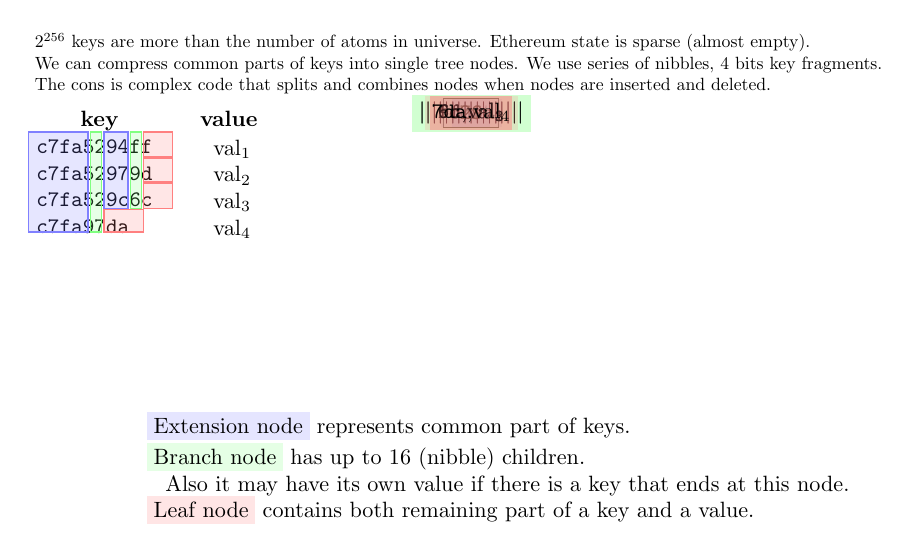
\begin{tikzpicture}[scale=0.8,every node/.style={transform shape}]

\node[align=left,anchor=north west,scale=0.8] at (0em,0ex) {
$2^{256}$ keys are more than the number of atoms in universe. Ethereum state is sparse (almost empty).\\
We can compress common parts of keys into single tree nodes. We use series of nibbles, 4 bits key fragments.\\
The cons is complex code that splits and combines nodes when nodes are inserted and deleted.};

\def\kx{0em}
\def\ky{-11ex}
\node[anchor=north west] at (\kx+2em,\ky+3ex) {\textbf{key}};
\node[anchor=north west] at (\kx+7.4em,\ky+3ex) {\textbf{value}};
\node[align=left,anchor=north west] at (\kx+8em,\ky) {
val\textsubscript{1}\\
val\textsubscript{2}\\
val\textsubscript{3}\\
val\textsubscript{4}};
\node[align=left,anchor=north west] at (\kx,\ky) {
\texttt{c7fa5294ff}\\
\texttt{c7fa52979d}\\
\texttt{c7fa529c6c}\\
\texttt{c7fa97da}};
\tikzstyle{key}=[fill,fill opacity=0.2,line width=0.6pt]
\draw[key,blue!50] (\kx,\ky) rectangle (\kx+2.7em,\ky-10.5ex);
\draw[key,green!50] (\kx+2.8em,\ky) rectangle (\kx+3.3em,\ky-10.5ex);
\draw[key,blue!50] (\kx+3.4em,\ky) rectangle (\kx+4.5em,\ky-8.0ex);
\draw[key,green!50] (\kx+4.6em,\ky) rectangle (\kx+5.1em,\ky-8.0ex);
\draw[key,red!50] (\kx+5.2em,\ky) rectangle (\kx+6.5em,\ky-2.6ex);
\draw[key,red!50] (\kx+5.2em,\ky-2.7ex) rectangle (\kx+6.5em,\ky-5.2ex);
\draw[key,red!50] (\kx+5.2em,\ky-5.3ex) rectangle (\kx+6.5em,\ky-8.0ex);
\draw[key,red!50] (\kx+3.4em,\ky-8.1ex) rectangle (\kx+5.2em,\ky-10.5ex);

\begin{scope}[xshift=20em,yshift=-9ex]
\tikzstyle{treenode}=[fill opacity=0.2,text opacity=1]
\tikzset{edge from parent/.style={draw,edge from parent path={(\tikzparentnode.south) -- +(0,-0.6ex) -| (\tikzchildnode.north)}}}
\Tree [ .\node[draw]{root}; [
  .\node[treenode,fill=blue!50]{\texttt{c7fa}}; [
    .\node[treenode,fill=green!50]{$|||||||||||||||||$};
      \edge node[auto=right]{\footnotesize{5}}; [ .\node[treenode,fill=blue!50]{\texttt{29}}; [
        .\node[treenode,fill=green!50]{$|||||||||||||||||$};
          \edge node[auto=right]{\footnotesize{4}}; \node[treenode,fill=red!50]{\texttt{ff},val\textsubscript{1}};
          \edge node[auto=right]{\footnotesize{7}}; \node[treenode,fill=red!50]{\texttt{9d},val\textsubscript{2}};
          \edge node[auto=left]{\footnotesize{c}}; \node[treenode,fill=red!50]{\texttt{6c},val\textsubscript{3}};
        ]
      ]
      \edge node[auto=left]{\footnotesize{9}}; \node[treenode,fill=red!50]{\texttt{7da},val\textsubscript{4}};
  ]
]]
\end{scope}

\node[align=left,anchor=north west] at (5em,-39.5ex) {
\colorbox{blue!10}{Extension node} represents common part of keys.\\
\colorbox{green!10}{Branch node} has up to 16 (nibble) children.\\
\hspace{0.5em} Also it may have its own value if there is a key that ends at this node.\\
\colorbox{red!10}{Leaf node} contains both remaining part of a key and a value.};

  \end{tikzpicture}
\end{frame}